% Define the type of document:
\documentclass{article}

\usepackage[utf8]{inputenc}
% Define the language:
\usepackage[spanish]{babel}

% Filler text and filler math:
\usepackage{blindtext}

% Margins
\usepackage[a4paper, inner=1.7cm, outer=4cm, top=2cm, bottom=2.5cm, bindingoffset=1.2cm, foot=0.25cm]{geometry}

% Margin notes
\usepackage{marginnote}

% Headers
\usepackage{fancyhdr}

% Replace the default sans-serif font with helvetica
\usepackage[scaled=.92]{helvet}

% To create lists and enumerations:
\usepackage{enumitem}  % Makes lists more compact

% Pictures
\usepackage{graphicx}  % Inclusion of images
\usepackage{wrapfig} % To wrap text around the pictures
\usepackage{subcaption} % Several pictures in one figure
 
% To write urls and link them with the pages:
\usepackage{hyperref}

% Improve justification
\usepackage{microtype}

% Tables
\usepackage{tabularx}

% Indexing
\usepackage{index}

% Math
\usepackage{amsmath}
\usepackage{amsfonts}
\usepackage{amsthm}
% Code
\usepackage{listings}

% Define some colors
\usepackage{color}

% Control pages
\usepackage{afterpage}

\definecolor{dkgreen}{rgb}{0,0.6,0}
\definecolor{gray}{rgb}{0.5,0.5,0.5}
\definecolor{mauve}{rgb}{0.58,0,0.82}
% Create a new style for the code
\lstdefinestyle{mystyle}{frame=tb,
  language=[LaTeX]{TeX},
  aboveskip=3mm,
  belowskip=3mm,
  showstringspaces=false,
  columns=flexible,
  basicstyle={\small\ttfamily},
  numbers=none,
  numberstyle=\tiny\color{gray},
  keywordstyle=\color{blue},
  commentstyle=\color{dkgreen},
  stringstyle=\color{mauve},
  breaklines=true,
  breakatwhitespace=true,
  tabsize=3
}

% Set it as the current style
\lstset{style=mystyle}

% Create some space between paragraphs
\setlength{\parskip}{0.3em}
\setlength{\parindent}{0pt}

\renewcommand{\headrulewidth}{0pt}  % Altura de la barra del header
\renewcommand{\footrulewidth}{1pt}  % Altura de la barra del footer


\title{\vspace{10em}\Huge Assignment 2: Queuing Theory \\\vspace{3cm}
\Large Advanced Networking}
\author{
Pablo Landrove Pérez-Gorgoroso}
\date{\Large March, 2026}

\begin{document}

% Página de título
\maketitle

\newpage
\clearpage

\section{Maximum Rate Possible}

\begin{figure}[h]
  \centering
  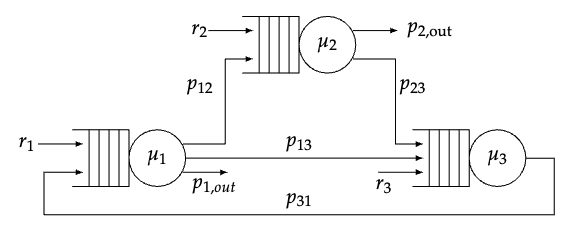
\includegraphics[width=0.6\textwidth]{Figures/porblem1.png}
  \caption{Queuing network diagram}
\end{figure}



Our goal is to find the maximum value for $r_1$ that maintains the stability of the system, that is $\lambda_i \leq \mu_i \; \forall i\in\{1,2,3\}$.

We define each arrival $\lambda_i$ rate as:

\begin{equation}
\lambda_i = r_i + \sum_{j=1}^3 p_{ji} \lambda_j
\end{equation}

We are given the following information:

\begin{itemize}
  \item The arrival rate from outside of the system for servers $2$ and $3$: $r_2=r_3=1$.
  \item Each routing probability $p_{ij}$.
  \item The processing rate of each server $\mu_i=10\,jobs/sec$
\end{itemize}

Given this information we can find the maximum rate $r_1$. We can model this as a linear programming problem, and since the optimum of a linear program is always achieved at a constraint boundary, we only need to check the value of $r_1$ when each constraint $\lambda_i \leq 10$ is saturated.

For each server $i$, we set $\lambda_i = 10$ and solve for $r_1$, keeping only the cases where all other constraints are also satisfied. The maximum value of $r_1$ across these cases is our answer.

\begin{equation}
  \begin{cases}
    \lambda_i \leq 10 \quad \forall i\in\{1,2,3\} \\
    \lambda_1 = r_1 + p_{31} \, \lambda_3= 1 + 0.8 \, \lambda_3 \\
    \lambda_2 = r_2 + p_{12} \, \lambda_1 = 1 + 0.8 \, \lambda_1 \\
    \lambda_3 = r_3 + p_{13} \, \lambda_1 + p_{23} \, \lambda_2 = 1 + 0.2 \, \lambda_1 + 0.2 \, \lambda_3
  \end{cases}
\end{equation}

\subsection{Saturate output of server 1}

\begin{equation}
  \begin{cases}
    \lambda_1=10 \\
    \lambda_2 = r_2 + p_{12} \, \lambda_1 = 9\\
    \lambda_3 = r_3 + p_{13} \, \lambda_1 + p_{23}\,\lambda_2 = 4.8 \\
    r_1 + p_{31}\,\lambda_3=10 \Rightarrow r_1 = 4.2\\
  \end{cases}
\end{equation}

All constraints are satisfied and we obtain that when $\lambda_1=10$, $r_1=4.2$.

\subsection{Saturate output of server 2}

\begin{equation}
  \lambda_2=r_2+p_{12}\,\lambda_1 =10 \Rightarrow \lambda_1 = 11.25
\end{equation}

If we saturate $\lambda_2$, we break the $\lambda_1$ constraint, so this is not a feasible solution.

\subsection{Saturate output of server 3}

\begin{equation}
  \lambda_3=r_3+p_{13}\,\lambda_1 + p_{23} \, \lambda_2 = 10 \Rightarrow \lambda_1 + \lambda_2 = 45
\end{equation}

The sum of $\lambda_1$ and $\lambda_2$ is 45, so one of them must be breaking the constraint, making this solution unfeasible.

\subsection{Optimal result}

If we saturate $\lambda_2$ or $\lambda_3$, we reach that some of the other constraints are not satisfied. Therefore, the optimal solution is obtained when saturating $\lambda_1$, with which we obtain $r_1=4.2$.

\section{Little's Theorem}

\subsection{Average occupation}

We can use Little's Theorem to obtain the average number of patients in the waiting room $N$, we have the mean waiting time $T=180$ minutes and the arrival rate $\lambda = 0.2$ patients/minute. So we obtain:

\begin{equation}
  N = \lambda T = 36 \text{ patients}
\end{equation}

\subsection{Size of the waiting room}

It is not possible to determine a waiting room size that will always accommodate all arrivals based solely on the given information. Patient arrivals are random, meaning there is no fixed upper bound on how many patients could arrive in a short period of time.

Therefore, in theory, an arbitrarily large number of patients could arrive, so no finite waiting room size can guarantee accommodation in all cases.
However, if additional information about the arrival distribution were provided, we could design the waiting room to handle demand with a specified confidence level.

\section{M/M/1 Queue Length}

Here $N_Q$ denotes the length of the queue. In the state $0$, there are no packets in the system, so the queue is empty. In the state $1$ too, as the arrived packet is in the server slot, so the queue is empty. For any state $i\geq2$, the length of the queue is $i-1$. So we can define the expectance of the queue length as:

\begin{equation}
  E[N_Q]=\sum_{i=2}^{+\infty}(i-1)P_i
\end{equation}

With $P_i$ the stationary probability of state $i$, using the development from the notes: $P_n=\rho^n P_0$ and that $P_0= (1-\rho)$, we arrive at the following:

\begin{align}
  E[N_Q]&=\sum_{i=2}^{+\infty}(i-1)\rho^i (1-\rho)=(1-\rho)\sum_{i=2}^{+\infty}(i-1)\rho^i=(1-\rho)\rho\sum_{i=2}^{+\infty}(i-1)\rho^{i-1}=\\
  &=(1-\rho)\rho\sum_{i=1}^{+\infty}i\rho^i=(1-\rho)\rho\sum_{i=0}^{+\infty}i\rho^i=\frac{\rho^2}{1-\rho}
\end{align}

\begin{figure}[h]
  \centering
  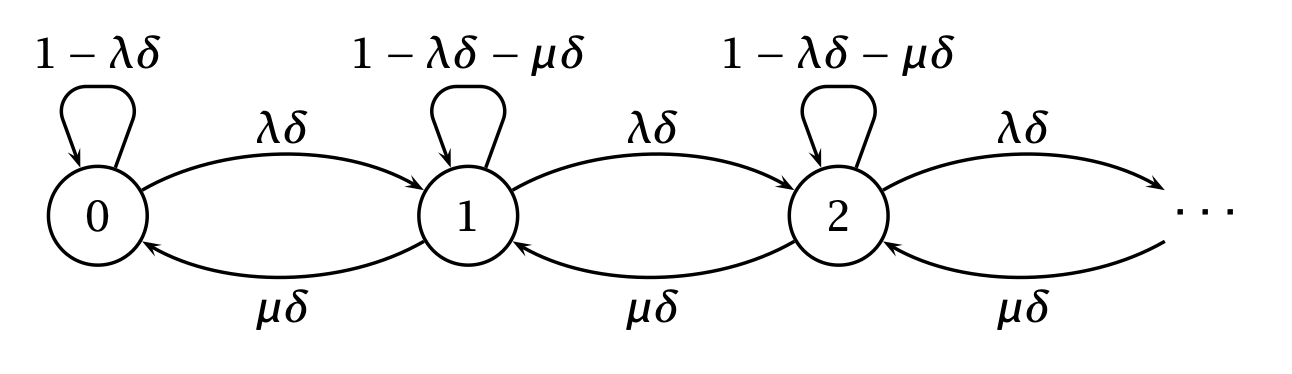
\includegraphics[width=0.6\textwidth]{Figures/markovmm1.png}
  \caption{M/M/1 Markov chain}
\end{figure}

\section{M/M/1 Queue}

We have packets arriving to a link at a rate of $450$ packets/sec, each having $500$ bytes on average. The link capacity link is $1$ Mbps.

\begin{equation}
1\text{Mbps} = 0.125\cdot10^6\,\text{bytes/sec}\Rightarrow 500\text{packets/sec}
\end{equation}

So we have the following information:

\begin{itemize}
  \item Arrival rate ($\lambda$): $450$ packets/sec.
  \item Service rate ($\mu$): $500$ packets/sec.
  \item Number of servers ($s$): 1.
  \item Utilization rate ($\rho$): $\frac{\lambda}{\mu}=0.9$.
\end{itemize}

\subsection{Queue length}

We need to obtain the probability that the queue has one, two or ten packets. That is that the probability that the system occupancy is two, three or eleven packets respectively ($P_2$, $P_3$ and $P_{10}$). We can use the expression from the last exercise: $P_n=\rho^n (1-\rho)$.

\begin{itemize}
  \item $P_2=\rho^2(1-\rho)=0.081$.
  \item $P_3=\rho^3(1-\rho)=0.0729$.
  \item $P_{11}=\rho^{11}(1-\rho)\approx0.0314$.
\end{itemize}

\subsection{Mean number of packets}

We can obtain the mean number of packets in the system as the expectance of the queue occupancy $n$:

\begin{equation}
  E[n]=\sum_{k=0}^{+\infty}kP_k=\sum_{k=1}^{+\infty}k\rho^k(1-\rho)=\frac{\rho}{1-\rho}=9
\end{equation}

And the mean number of packets in the queue as the expectance of $N_Q$:

\begin{equation}
  E[N_Q]=\frac{\rho^2}{1-\rho}=8.1
\end{equation}

\subsection{Mean waiting time}

We can obtain this using Little's theorem, given mean number of packets in the queue $E[N_Q]$ and the arrival rate $\lambda$:

\begin{equation}
  T=\frac{E[N_Q]}{\lambda}=0.018 \text{ sec}
\end{equation}

% SECCIONES
\pagestyle{fancy}
\fancyhead{}
\pagenumbering{arabic}

\end{document}
